\documentclass{article}
\usepackage{amsmath}
\usepackage[mathletters]{ucs}
\usepackage[utf8x]{inputenc}
\usepackage[margin=1.5in]{geometry}
\usepackage{enumerate}
\newtheorem{theorem}{Theorem}
\usepackage[dvipsnames]{xcolor}
\usepackage{pgfplots}
\setlength{\parindent}{0cm}
\usepackage{graphics}
\usepackage{graphicx} % Required for including images
\usepackage{subcaption}
\usepackage{bigintcalc}
\usepackage{pythonhighlight} %for pythonkode \begin{python}   \end{python}
\usepackage{appendix}
\usepackage{arydshln}
\usepackage{physics}
\usepackage{tikz-cd}
\usepackage{booktabs} 
\usepackage{adjustbox}
\usepackage{mdframed}
\usepackage{relsize}
\usepackage{physics}
\usepackage[thinc]{esdiff}
\usepackage{fixltx2e}
\usepackage{esint}  %for lukket-linje-integral
\usepackage{xfrac} %for sfrac
\usepackage{hyperref} %for linker, må ha med hypersetup
\usepackage[noabbrev, nameinlink]{cleveref} % to be loaded after hyperref
\usepackage{amssymb} %\mathbb{R} for reelle tall, \mathcal{B} for "matte"-font
\usepackage{listings} %for kode/lstlisting
\usepackage{verbatim}
\usepackage{graphicx,wrapfig,lipsum,caption} %for wrapping av bilder
\usepackage{mathtools} %for \abs{x}
\usepackage[norsk]{babel}
\definecolor{codegreen}{rgb}{0,0.6,0}
\definecolor{codegray}{rgb}{0.5,0.5,0.5}
\definecolor{codepurple}{rgb}{0.58,0,0.82}
\definecolor{backcolour}{rgb}{0.95,0.95,0.92}

\lstdefinestyle{mystyle}{
    backgroundcolor=\color{backcolour},   
    commentstyle=\color{codegreen},
    keywordstyle=\color{magenta},
    numberstyle=\tiny\color{codegray},
    stringstyle=\color{codepurple},
    basicstyle=\ttfamily\footnotesize,
    breakatwhitespace=false,         
    breaklines=true,                 
    captionpos=b,                    
    keepspaces=true,                 
    numbers=left,                    
    numbersep=5pt,                  
    showspaces=false,                
    showstringspaces=false,
    showtabs=false,                  
    tabsize=2
}

\lstset{style=mystyle}
\author{Oskar Idland}
\title{FYS1120 Linjer på Kryss og Tvers}
\date{}
\begin{document}
\maketitle
\newpage

\section*{a)}
  Ved bruk av superposisjons prinsippet vet vi at feltene skapt av linjeladingene langs x og z-aksen kan kombineres for å finne feltet i xy-planet. Vi har allerede fått likningen for feltet til linjeladningen som går langs z-aksen og kan gjøre den om slik at den passer for ladningen langs x-aksen. Den eneste forskjellen er fortegnet på ladningstettheten, og retningsvektoren som nå skal stå radielt ut fra x-aksen. 
  \[
  \mathbf{E}_{z} = \frac{(Q / L)}{2 \pi \epsilon_0 r_1} \mathbf{\hat{r}}_{1}, \quad \mathbf{\hat{r}}_1 = (x, y, 0) \qquad \mathbf{E}_{x} = \frac{(-Q / L)}{2 \pi \epsilon_0 r_2} \mathbf{\hat{r}}_{2}, \quad \mathbf{\hat{r}}_2 = (0, y, z)
  \]
  \[
  \mathbf{E} = \mathbf{E}_{z} + \mathbf{E}_{x} = \frac{Q / L}{2 \pi \epsilon_{0}} \left( \frac{\mathbf{\hat{r}}_{1}}{r_1} - \frac{\mathbf{\hat{r}_2}}{r_2} \right)_{}^{}
  \]

\section*{b)}
  Vi bruker superposisjons prinsippet og legger sammen feltet skapt av linjeladningene. Ettersom den ene linjen går gjennom $ (0,a) $ må retningsvektoren justeres. $ \mathbf{\hat{r}} = (x, y) - (x,5) = (0,-5) $
  \[
    \mathbf{E}_{x_0} = \frac{(-Q / L)}{2 \pi \epsilon_0 r_0} \mathbf{\hat{r}}_{0}, \quad \mathbf{\hat{r}}_0 = (0, y) \qquad \mathbf{E}_{x_5} = \frac{(-Q / L)}{2 \pi \epsilon_0 r_5} \mathbf{\hat{r}}_{5}, \quad \mathbf{\hat{r}}_5 = (0, y - 5)
  \]
  Vi får følgende plot:
  \begin{figure}[h!]
    \centering
    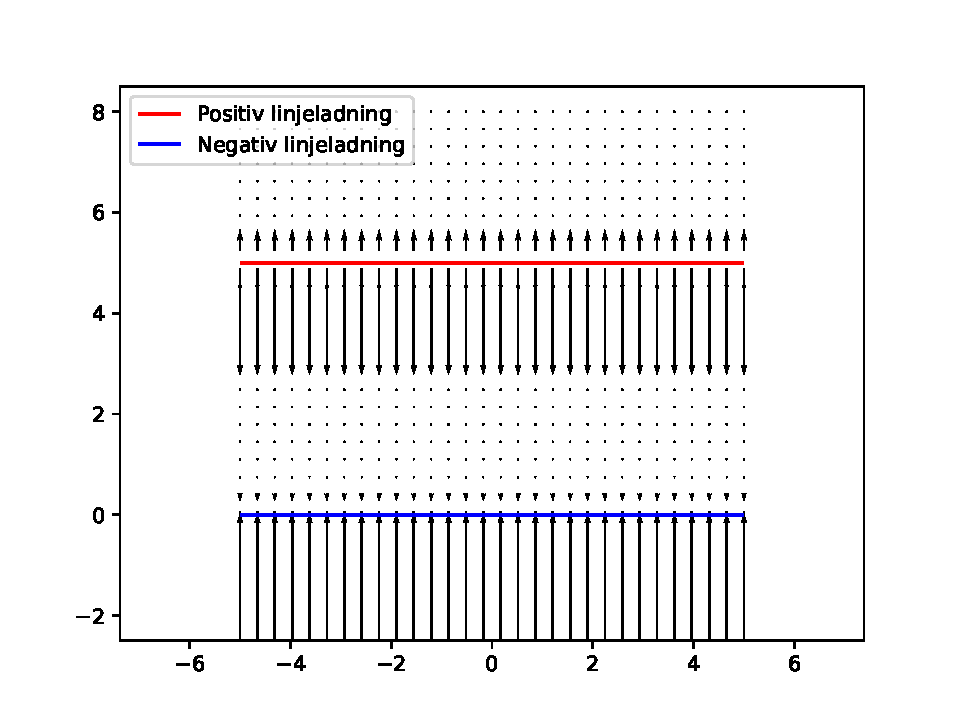
\includegraphics[scale = .45]{Linjeladninger_.b.pdf}
    \caption{Plot av to horisontale linjeladninger}
    \label{fig:figure2}
  \end{figure}

  Ved å bruke \nameref{Kode_b}:


\section*{c)}
  Vi bruker superposisjons prinsippet ved å legge sammen feltene fra begge linjeladningene for å finne det totalet elektriske feltet i xy-planet. Ettersom vi ser på xy-planet vil z komponenten være irrelevant og vi forenkler derfor formelene fra tidligere. 
  \[
  \mathbf{E}_x = \frac{(Q / L)}{2 \pi \epsilon_0 r_x} \mathbf{\hat{r}}_{x}, \quad \mathbf{\hat{r}}_x = (0, y) \qquad \mathbf{E}_{y} = \frac{(-Q / L)}{2 \pi \epsilon_0 r_y} \mathbf{\hat{r}}_{y}, \quad \mathbf{\hat{r}}_y = (x, 0)
  \]
  Vi får følgende plot: 
  \begin{figure}[h!]
    \centering
    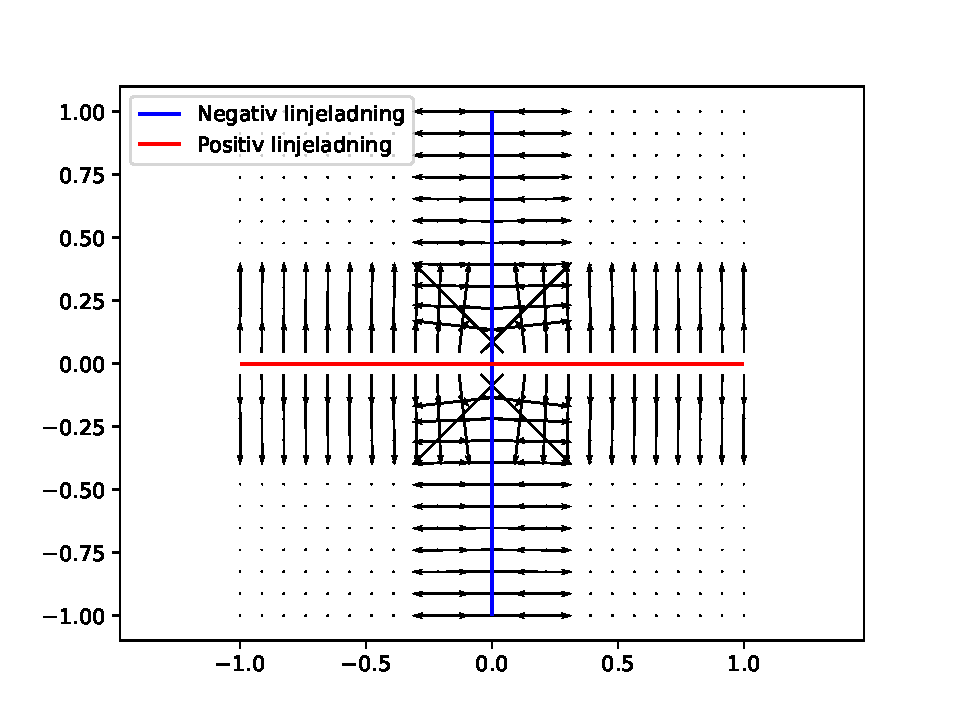
\includegraphics[scale = .4]{Linjeladninger_c.pdf}
    \caption{Plot av to linjeladninger langs x og y-aksen}
    \label{fig:figure1}
  \end{figure}

  Når vi kjører \nameref{Kode_c}:




  \lstinputlisting[label = {Kode_b}, caption = {kode tillhørende oppgave b}, language = python]{ Linjeladninger_b.py}  
  

  \lstinputlisting[label = {Kode_c}, caption = {kode tillhørende oppgave c}, language = python]{ Linjeladninger_c.py}  

\end{document}